\documentclass[letterpaper,titlepage,oneside]{article}
\setlength\parindent{24pt}
\usepackage{listings}
\usepackage{graphicx}
\usepackage{color}

\definecolor{dkgreen}{rgb}{0,0.6,0}
\definecolor{gray}{rgb}{0.5,0.5,0.5}
\definecolor{mauve}{rgb}{0.58,0,0.82}

\lstset{frame=tb,
  language=Java,
  aboveskip=3mm,
  belowskip=3mm,
  showstringspaces=false,
  columns=flexible,
  basicstyle={\small\ttfamily},
  numbers=none,
  numberstyle=\tiny\color{gray},
  keywordstyle=\color{blue},
  commentstyle=\color{dkgreen},
  stringstyle=\color{mauve},
  breaklines=true,
  breakatwhitespace=true,
  tabsize=4
}


\begin{document}


\begin{center}
\section*{THE COOPER UNION \\FOR THE ADVANCEMENT OF SCIENCE AND ART\\[35pt]}
\section*{A Practical Method for the Implementation of \\Cascading Tetrominoes with Digital Logic\\[35pt]}
\subsection*{Arnold Wey, EE '18 \\[15pt]-\&-\\[15pt] Camilo Gaitan, CE '18\\[75pt]}
\subsection*{A thesis submitted in partial fulfillment of the requirements for the degree of Bachelor of Engineering\\[75pt]}
\subsubsection*{May 13, 2015\\[60pt]}
\subsubsection*{Professor Jared Harwayne-Gidansky\\[5pt]Thesis Advisor}
\end{center}
\pagebreak
\tableofcontents
\pagebreak
\pagestyle{headings}
\section{Abstract}
The objective of the project is a digital logic port of the 1984 game Tetris, which involves the manipulation of a falling shape in a vertical board. Key features of gameplay are the random generation of falling Tetrominoes, the ability to move the falling shape (henceforth referred to as "Mino") left, right, and rotate it, and the deletion of full lines. 

Tetrominoes are hard coded into an EEPROM, which is addressed by counters controlled by buttons.

The Field itself is rendered row-by-row from the bottom up, while processing each row and checking for a full row, an empty row, and selecting either the current row or the next row to write into RAM. The bottom row of the mino, RowBottom, corresponds to its location in the board and is compared with the current row being processed, which determines whether to enable the output of the corresponding row from the EEPROM. This RowBottom is maintained by a 3-bit down counter.

The output is displayed by sinking current on 1 row of the LED matrix at a time, while sourcing power to the appropriate "x" ordinates. \\
This happens at a high frequency; the frame looks whole via persistence of vision.

The project demonstrates the basic functionality of Tetris. Additional safeguards could be implemented but weren't defined in the project specs, such as Left/Right collision detection, wall collision detection, increased falling speed as the game progresses, and scoring system.
\pagebreak
\section{Design Considerations}

These solutions were devised through an iterative process which slowly decreased the number of boards required to implement Tetris. The original design required over 30 boards, which has slowly been trimmed down to around 14. 

Tetris has been traditionally implemented on a 10x20 board, which was an awkward number of inputs to MUX, and required an extra chip for every part of the circuit that used MUXs, as well as 3 4-bit shift registers instead of 2. What made this factor even worse was the original implementation to display the board.

Originally, the Tetromino would be loaded into a RAM separate from the RAM storing the FIELD. The outputs from the two RAMs would be time-domain MUXed to individual LEDs. Reducing the board to 8x16 brought the board count to 24. 

Then, we considered loading each shape into 4 8-bit Universal Shift Registers (8 4-bit SRs), which could be manipulated and fed into rotation matrices in order to manipulate the output. 

While building, we realized that hard-coding the possible states of each row containing a Tetromino could fit inside the EEPROM, completely eliminating the need for the 4 shift registers storing each row that would handle shifting left and right, not to mention save the cost of Universal Shift Registers, which are quite costly. \\
This brought the total board count to around 18, but required writing 1024 unique rows

The need to manually write 1024 bytes prompted an investigation in automating the process. There's no simple way to handle rotation, so\\
$ 4 rows * 8 shapes * 4 orientations = 128 rows$
were written manually into input.txt

shapeTest.c prints out all the possible offsets of each shape's orientations, read from input.txt. The stdout from shapeTest is redirected into Swag.txt. The debugging output is manually cleaned up, and used as input to bintext2bin.\\
bintext2bin.c converts input from a text file containing 8bit rows encoded as ASCII 1's and 0's into a bin file with equivalent information. (output.bin)\\
This bin file was loaded into the memory buffer at even addresses, for pinning convenience. Additionally, this allows the LSB on the EEPROM to be used as a logical disable.

Asserting 1 row at a time from the EEPROM and the RAM allows us to do away with another set of MUXs, and performing a bit-wise OR to control the display.

After cutting down the number of boards required to control the shape, we needed to reexamine the logic handling the RAM.

In order to access and manipulate information within the RAM, they must be stored and displayed on Shift Registers. [INSERT SHIFT REGISTER IMPLEMENTATION AND FLAG-RAISING]

Writing back into the RAM requires having read and write information asserted on the same bus. This requires the use of a Tri-State enabled MUX.


\pagebreak
A few more boards were saved by implementing Truth Table~\ref{table:OverLap_Unminimized} on page~\pageref{table:OverLap_Unminimized}
 into a GAL chip, Overlap.
 
That Truth Table simplifies into Truth Table~\ref{table:Overlap_Minimized} on page~\pageref{table:Overlap_Minimized}, and results in the following Equivalent Expression:\\[5pt]
$Overlap=(B2+B3+B4+!A2)*(B2+B3+!A2+!A4)*(B2+B3+!A2+!A3)*\\
(B2+B4+!A2+!A3)*(B2+!A2+!A3+!A4)*(!B1+A1)*(B1+!A1+!A2)*\\
(!B2+A1+A2)*(B1+B2+!A1)*(B2+!B3+A2+A3)*(!B2+B3+B4+A2)*\\
*(!B2+A2+!A3+!A4)*(!B2+!B3+!A2+A3)*(B2+!B3+!B4+A2+A4)*\\
(B2+!B4+A2+A3+A4)*(!B2+B3+A2+!A3)*(!B2+B3+A2+!A4)*\\
(!B2+B4+A2+!A3)*(!B2+!B3+!B4+!A2+A4)*(!B2+!B4+!A2+A3+A4)$\\

This had few enough product terms to fit onto a GAL16v8, and upon securing approval, we programmed the chip using WinCUPL and the ChipMaster 6000 graciously provided to us by the Cooper Union Electrical Engineering Department.

The Overlap.PLD source code, followed by snippets of the test vector file, can be found on page~\pageref{code:Overlap}.

\pagebreak
\section{Sample Code}

\paragraph*{Overlap.PLD\\}
\label{code:Overlap}
\begin{lstlisting}
Name 	Overlap;
Partno 	01;
Date 	4/24/2015;
Rev 	01;
Designer 	Arnold Wey;
Company 	CU Later;
Assembly 	None;
Location 	None;
Device 	g16v8;

/**Inputs**/
Pin 1 = A1;
Pin 2 = A2;
Pin 3 = A3;
Pin 4 = A4;
Pin 5 = B1;
Pin 6 = B2;
Pin 7 = B3;
Pin 8 = B4;

/**Outputs**/
Pin 15 = I1;
Pin 16 = I2;
Pin 17 = I3;
Pin 18 = I4;
Pin 14 = Overlap;
Pin 13 = NotOverlap;
O0 = B2#B3#B4#!A2;
O1 = B2#B3#!A2#!A4;
O2 = B2#B3#!A2#!A3;
O3 = B2#B4#!A2#!A3;
O4 = B2#!A2#!A3#!A4;
O5 = !B1#A1;
O6 = B1#!A1#!A2;
O7 = !B2#A1#A2;
O8 = B1#B2#!A1;
O9 = B2#!B3#A2#A3;
O10 = !B2#B3#B4#A2;
O11 = !B2#A2#!A3#!A4;
O12 = !B2#!B3#!A2#A3;
O13 = B2#!B3#!B4#A2#A4;
O14 = B2#!B4#A2#A3#A4;
O15 = !B2#B3#A2#!A3;
O16 = !B2#B3#A2#!A4;
O17 = !B2#B4#A2#!A3;
O18 = !B2#!B3#!B4#!A2#A4;
O19 = !B2#!B4#!A2#A3#A4;

/*Combining Terms*/
I1 = [O0, O1, O2, O3, O4, O10,O15]: & ;
I2 = [O5, O6, O7, O8, O9]: & ;
I3 = [O11,O13]: & ;
I4 = [O16,O17,O18,O19]: & ;

/*Final Terms*/
Overlap = [I1, I2, I3, I4,O14,O12]: & ;
NotOverlap = !Overlap;
\end{lstlisting}

\subsection*{Overlap.SI}
\label{code:OverlapSi}
\begin{lstlisting}

Name     	Overlap;
PartNo   	01;
Date     	4/24/2015;
Revision 	01;
Designer 	Arnold Wey;
Company  	CU Later;
Assembly 	None;
Location 	None;
Device   	g16v8;

ORDER: B1, B2, B3, B4, A1, A2, A3, A4, Overlap, NotOverlap; 

VECTORS:
00000000HL
00000001HL
00000010HL
00000011HL
00000100LH
00000101LH
00000110LH
00000111LH
00001000LH
   ...

\end{lstlisting}

\pagebreak
\subsection*{8AndNor.PLD}
\label{code: 8AndNor}
\begin{lstlisting}
Name 4bSel;
Partno 01;
Date 4/15/2015;
Rev 01;
Designer Arnold Wey;
Company CU Later;
Assembly None;
Location None;
Device g22v10;

/**Inputs**/
Pin 1 = ADD;

Pin 4 = A0;
Pin 5 = A1;
Pin 6 = A2;
Pin 7 = A3;
Pin 8 = B0;
Pin 9 = B1;
Pin 10 = B2;
Pin 11 = B3;

/**Outputs**/
Pin 18 = Y3;
Pin 19 = Y2;
Pin 20 = Y1;
Pin 21 = Y0;

Y0 = A0  &  !ADD;
APPEND Y0 = B0  &  ADD;
Y1 = A1  &  !ADD;
APPEND Y1 = B1  &  ADD;
Y2 = A2  &  !ADD;
APPEND Y2 = B2  &  ADD;
Y3 = A3  &  !ADD;
APPEND Y3 = B3  &  ADD;
\end{lstlisting}
\pagebreak
\paragraph*{8AndNor.SI}
\label{code: 8AndNorSi}
\begin{lstlisting}
Name     8AndNor;
PartNo   01;
Date     4/15/2015;
<Revision></Revision>;
Designer Arnold Wey;
Company  CU Later;
Assembly None;
Location None;
Device   g16v8;


ORDER: I7, I6, I5, I4, I3, I0, I1, I2, AND, OR; 


VECTORS:
00000000LL
00000001LH
00000010LH
00000011LH
00000100LH
00000101LH
00000110LH
00000111LH
00001000LH
00001001LH
00001010LH
00001011LH
00001100LH
   ...
\end{lstlisting}

\pagebreak
\paragraph*{4BSel.PLD}
\label{code: 4BSel}
\begin{lstlisting}
Name 4bSel;
Partno 01;
Date 4/15/2015;
Rev 01;
Designer Arnold Wey;
Company CU Later;
Assembly None;
Location None;
Device g22v10;
/**Inputs**/
Pin 1 = ADD;

Pin 4 = A0;
Pin 5 = A1;
Pin 6 = A2;
Pin 7 = A3;
Pin 8 = B0;
Pin 9 = B1;
Pin 10 = B2;
Pin 11 = B3;
/**Outputs**/

Pin 18 = Y3;
Pin 19 = Y2;
Pin 20 = Y1;
Pin 21 = Y0;

Y0 = A0  &  !ADD;
APPEND Y0 = B0  &  ADD;
Y1 = A1  &  !ADD;
APPEND Y1 = B1  &  ADD;
Y2 = A2  &  !ADD;
APPEND Y2 = B2  &  ADD;
Y3 = A3  &  !ADD;
APPEND Y3 = B3  &  ADD;
\end{lstlisting}
\pagebreak
\paragraph*{4BSel.SI}
\label{code: 4BSelSi}
\begin{lstlisting}
Name     4bSel;
PartNo   01;
Date     4/15/2015;
<Revision></Revision>;
Designer Arnold Wey;
Company  CU Later;
Assembly None;
Location None;
Device   g22v10;


ORDER: A0, ADD, B0, A1, B1, A2, B2, A3, B3, Y0, Y1, Y2, Y3; 


VECTORS:
000000000LLLL
000000001LLLL
000000010LLLH
000000011LLLH
000000100LLLL
000000101LLLL
000000110LLLH
000000111LLLH
000001000LLHL
000001001LLHL
000001010LLHH
000001011LLHH
000001100LLHL
000001101LLHL
000001110LLHH
000001111LLHH
\end{lstlisting}


\pagebreak
\section{Tables}

\subsection*{Overlap, Unminimized}
\begin{center}
\begin{table}['h']
\begin{tabular}{c|c|c|c|c|c|c|c|c|c|c|c}
\cline{2-11}

 & B1 & B2 & B3 & B4 & A1 & A2 & A3 & A4 & Overlap & !Overlap & \\ \cline{2-11}
 & 0 & 0 & 0 & 0 & 0 & 0 & 0 & 0 & H & L &   \\
 & 0 & 0 & 0 & 0 & 0 & 0 & 0 & 1 & H & L &   \\
 & 0 & 0 & 0 & 0 & 0 & 0 & 1 & 0 & H & L &   \\
 & 0 & 0 & 0 & 0 & 0 & 0 & 1 & 1 & H & L &   \\
 & 0 & 0 & 0 & 0 & 0 & 1 & 0 & 0 & L & H &   \\
 & 0 & 0 & 0 & 0 & 0 & 1 & 0 & 1 & L & H &   \\
 & 0 & 0 & 0 & 0 & 0 & 1 & 1 & 0 & L & H &   \\
 & 0 & 0 & 0 & 0 & 0 & 1 & 1 & 1 & L & H &   \\
 & 0 & 0 & 0 & 0 & 1 & 0 & 0 & 0 & L & H &   \\
 & 0 & 0 & 0 & 0 & 1 & 0 & 0 & 1 & L & H &   \\
 & 0 & 0 & 0 & 0 & 1 & 0 & 1 & 0 & L & H &   \\
 & 0 & 0 & 0 & 0 & 1 & 0 & 1 & 1 & L & H &   \\
 & 0 & 0 & 0 & 0 & 1 & 1 & 0 & 0 & L & H &   \\
 & 0 & 0 & 0 & 0 & 1 & 1 & 0 & 1 & L & H &   \\
 & 0 & 0 & 0 & 0 & 1 & 1 & 1 & 0 & L & H &   \\
 & 0 & 0 & 0 & 0 & 1 & 1 & 1 & 1 & L & H &   \\
 & 0 & 0 & 0 & 1 & 0 & 0 & 0 & 0 & L & H &   \\
 & 0 & 0 & 0 & 1 & 0 & 0 & 0 & 1 & H & L &   \\
 & 0 & 0 & 0 & 1 & 0 & 0 & 1 & 0 & H & L &   \\
 & 0 & 0 & 0 & 1 & 0 & 0 & 1 & 1 & H & L &   \\
 & 0 & 0 & 0 & 1 & 0 & 1 & 0 & 0 & H & L &   \\
 & 0 & 0 & 0 & 1 & 0 & 1 & 0 & 1 & L & H &   \\
 & 0 & 0 & 0 & 1 & 0 & 1 & 1 & 0 & L & H &   \\
 & \ldots & \ldots & \ldots & \ldots & \ldots & \ldots & \ldots & \ldots & \ldots & \ldots &  \\

\cline{2-11}
\end{tabular}
\caption{Abbreviated}\label{table:OverLap_Unminimized}
\end{table}


\end{center}


\pagebreak
\subsection*{Overlap, Minimized}

\begin{center}
\begin{table}['h']
\begin{tabular}{c|c|c|c|c|c|c|c|c|c|c}
\cline{2-10}
 & A1 & A2 & A3 & A4 & B1 & B2 & B3 & B4 & Overlap &  \\ \cline{2-10}
 & 1 & 1 & 0 & 0 & 1 & 1 & X & X & 1 &  \\
 & 0 & 1 & 0 & 0 & 0 & 1 & X & X & 1 &  \\
 & 1 & 0 & 0 & 0 & 1 & 0 & X & X & 1 &  \\
 & 0 & 0 & 0 & 0 & 0 & 0 & X & X & 1 &  \\
 & 1 & 1 & 0 & X & 1 & 1 & 1 & X & 1 &  \\
 & 1 & 1 & X & 0 & 1 & 1 & 1 & X & 1 &  \\
 & 0 & 1 & X & 0 & 0 & 1 & 1 & X & 1 &  \\
 & 1 & 0 & 0 & X & 1 & 0 & 1 & X & 1 &  \\
 & 1 & 0 & X & 0 & 1 & 0 & 1 & X & 1 &  \\
 & 0 & 0 & 0 & X & 0 & 0 & 1 & X & 1 &  \\
 & 0 & 0 & X & 0 & 0 & 0 & 1 & X & 1 &  \\
 & 1 & 0 & 1 & X & 1 & 1 & 0 & X & 1 &  \\
 & 0 & 0 & 1 & X & 0 & 1 & 0 & X & 1 &  \\
 & 1 & 1 & 0 & X & 1 & 1 & X & 1 & 1 &  \\
 & 1 & 0 & 0 & X & 1 & 0 & X & 1 & 1 &  \\
 & 0 & 0 & 0 & X & 0 & 0 & X & 1 & 1 &  \\
 & 1 & 1 & X & X & 1 & 1 & 1 & 1 & 1 &  \\
 & 1 & 0 & X & X & 1 & 0 & 1 & 1 & 1 &  \\
 & 0 & X & 1 & 1 & 0 & 1 & X & 0 & 1 &  \\
 & 0 & 1 & 1 & 0 & 1 & 0 & 0 & X & 1 &  \\
 & 0 & X & 1 & 1 & 0 & 0 & 1 & 1 & 1 &  \\
 & 1 & 0 & 1 & 1 & 1 & 1 & X & 0 & 1 &  \\
 & 1 & 0 & X & 1 & 1 & 1 & 0 & 0 & 1 &  \\
 & 0 & 0 & X & 1 & 0 & 1 & 0 & 0 & 1 &  \\
 & 0 & 1 & 0 & 1 & 1 & 0 & 0 & 0 & 1 &  \\
 & 0 & 1 & 0 & X & 0 & 1 & 1 & X & 1 &  \\
 & 0 & 1 & X & 1 & 0 & 1 & 0 & 1 & 1 &  \\
\cline{2-10}
\end{tabular}
\caption{Overlap, Minimized}\label{table:Overlap_Minimized}
\end{table}
\end{center}
\pagebreak

\subsection*{4BSel, Unminimized}

\begin{center}
\begin{table}['h']
\begin{tabular}{c|c|c|c|c|c|c|c|c|c|c|c|c|c|c}
\cline{2-14}
 & A0 & ADD & B0 & A1 & B1 & A2 & B2 & A3 & B3 & Y0 & Y1 & Y2 & Y3 &  \\ \cline{2-14}

 & 0 & 0 & 0 & 0 & 0 & 0 & 0 & 0 & 0 & L & L & L & L\\
 & 0 & 0 & 0 & 0 & 0 & 0 & 0 & 0 & 1 & L & L & L & L\\
 & 0 & 0 & 0 & 0 & 0 & 0 & 0 & 1 & 0 & L & L & L & H\\
 & 0 & 0 & 0 & 0 & 0 & 0 & 0 & 1 & 1 & L & L & L & H\\
 & 0 & 0 & 0 & 0 & 0 & 0 & 1 & 0 & 0 & L & L & L & L\\
 & 0 & 0 & 0 & 0 & 0 & 0 & 1 & 0 & 1 & L & L & L & L\\
 & 0 & 0 & 0 & 0 & 0 & 0 & 1 & 1 & 0 & L & L & L & H\\
 & 0 & 0 & 0 & 0 & 0 & 0 & 1 & 1 & 1 & L & L & L & H\\
 & 0 & 0 & 0 & 0 & 0 & 1 & 0 & 0 & 0 & L & L & H & L\\
 & 0 & 0 & 0 & 0 & 0 & 1 & 0 & 0 & 1 & L & L & H & L\\
 & 0 & 0 & 0 & 0 & 0 & 1 & 0 & 1 & 0 & L & L & H & H\\
 & \ldots{} & \ldots{} & \ldots{} & \ldots{} & \ldots{} & \ldots{} & %
\ldots{} & \ldots{} & \ldots{} & \ldots{} & \ldots{} & \ldots{} & \\
\cline{2-14}
\end{tabular}
\caption{Abbreviated}\label{table:4BSel_Unminimized}
\end{table}
\end{center}

\subsection*{8AndOr, Unminimized}

\begin{center}
\begin{table}['h']
\begin{tabular}{c|c|c|c|c|c|c|c|c|c|c|c|c}
\cline{2-11}
& I7 & I6 & I5 & I4 & I3 & I0 & I1 & I2 & AND & OR \\ 
\cline{2-11}
& 0 & 0 & 0 & 0 & 0 & 0 & 0 & 0 & L & L  \\  
& 0 & 0 & 0 & 0 & 0 & 0 & 0 & 1 & L & H \\
& 0 & 0 & 0 & 0 & 0 & 0 & 1 & 0 & L & H \\
& 0 & 0 & 0 & 0 & 0 & 0 & 1 & 1 & L & H \\
& 0 & 0 & 0 & 0 & 0 & 1 & 0 & 0 & L & H \\
& 0 & 0 & 0 & 0 & 0 & 1 & 0 & 1 & L & H \\
& \ldots{} & \ldots{} & \ldots{} & \ldots{} & \ldots{} & \ldots{} & %
\ldots{} & \ldots{} & \ldots{} & \ldots{}\\
& 1 & 1 & 1 & 1 & 1 & 1 & 1 & 0 & L & H \\
& 1 & 1 & 1 & 1 & 1 & 1 & 1 & 1 & H & H \\
\cline{2-11}
\end{tabular}
\caption{Abbreviated}\label{8AndOr_Unminimized}
\end{table}
\end{center}


\pagebreak

\section{Figures}

\subsection*{Collision Logic.sch}
\begin{center}
\begin{figure}[hp]
\centering
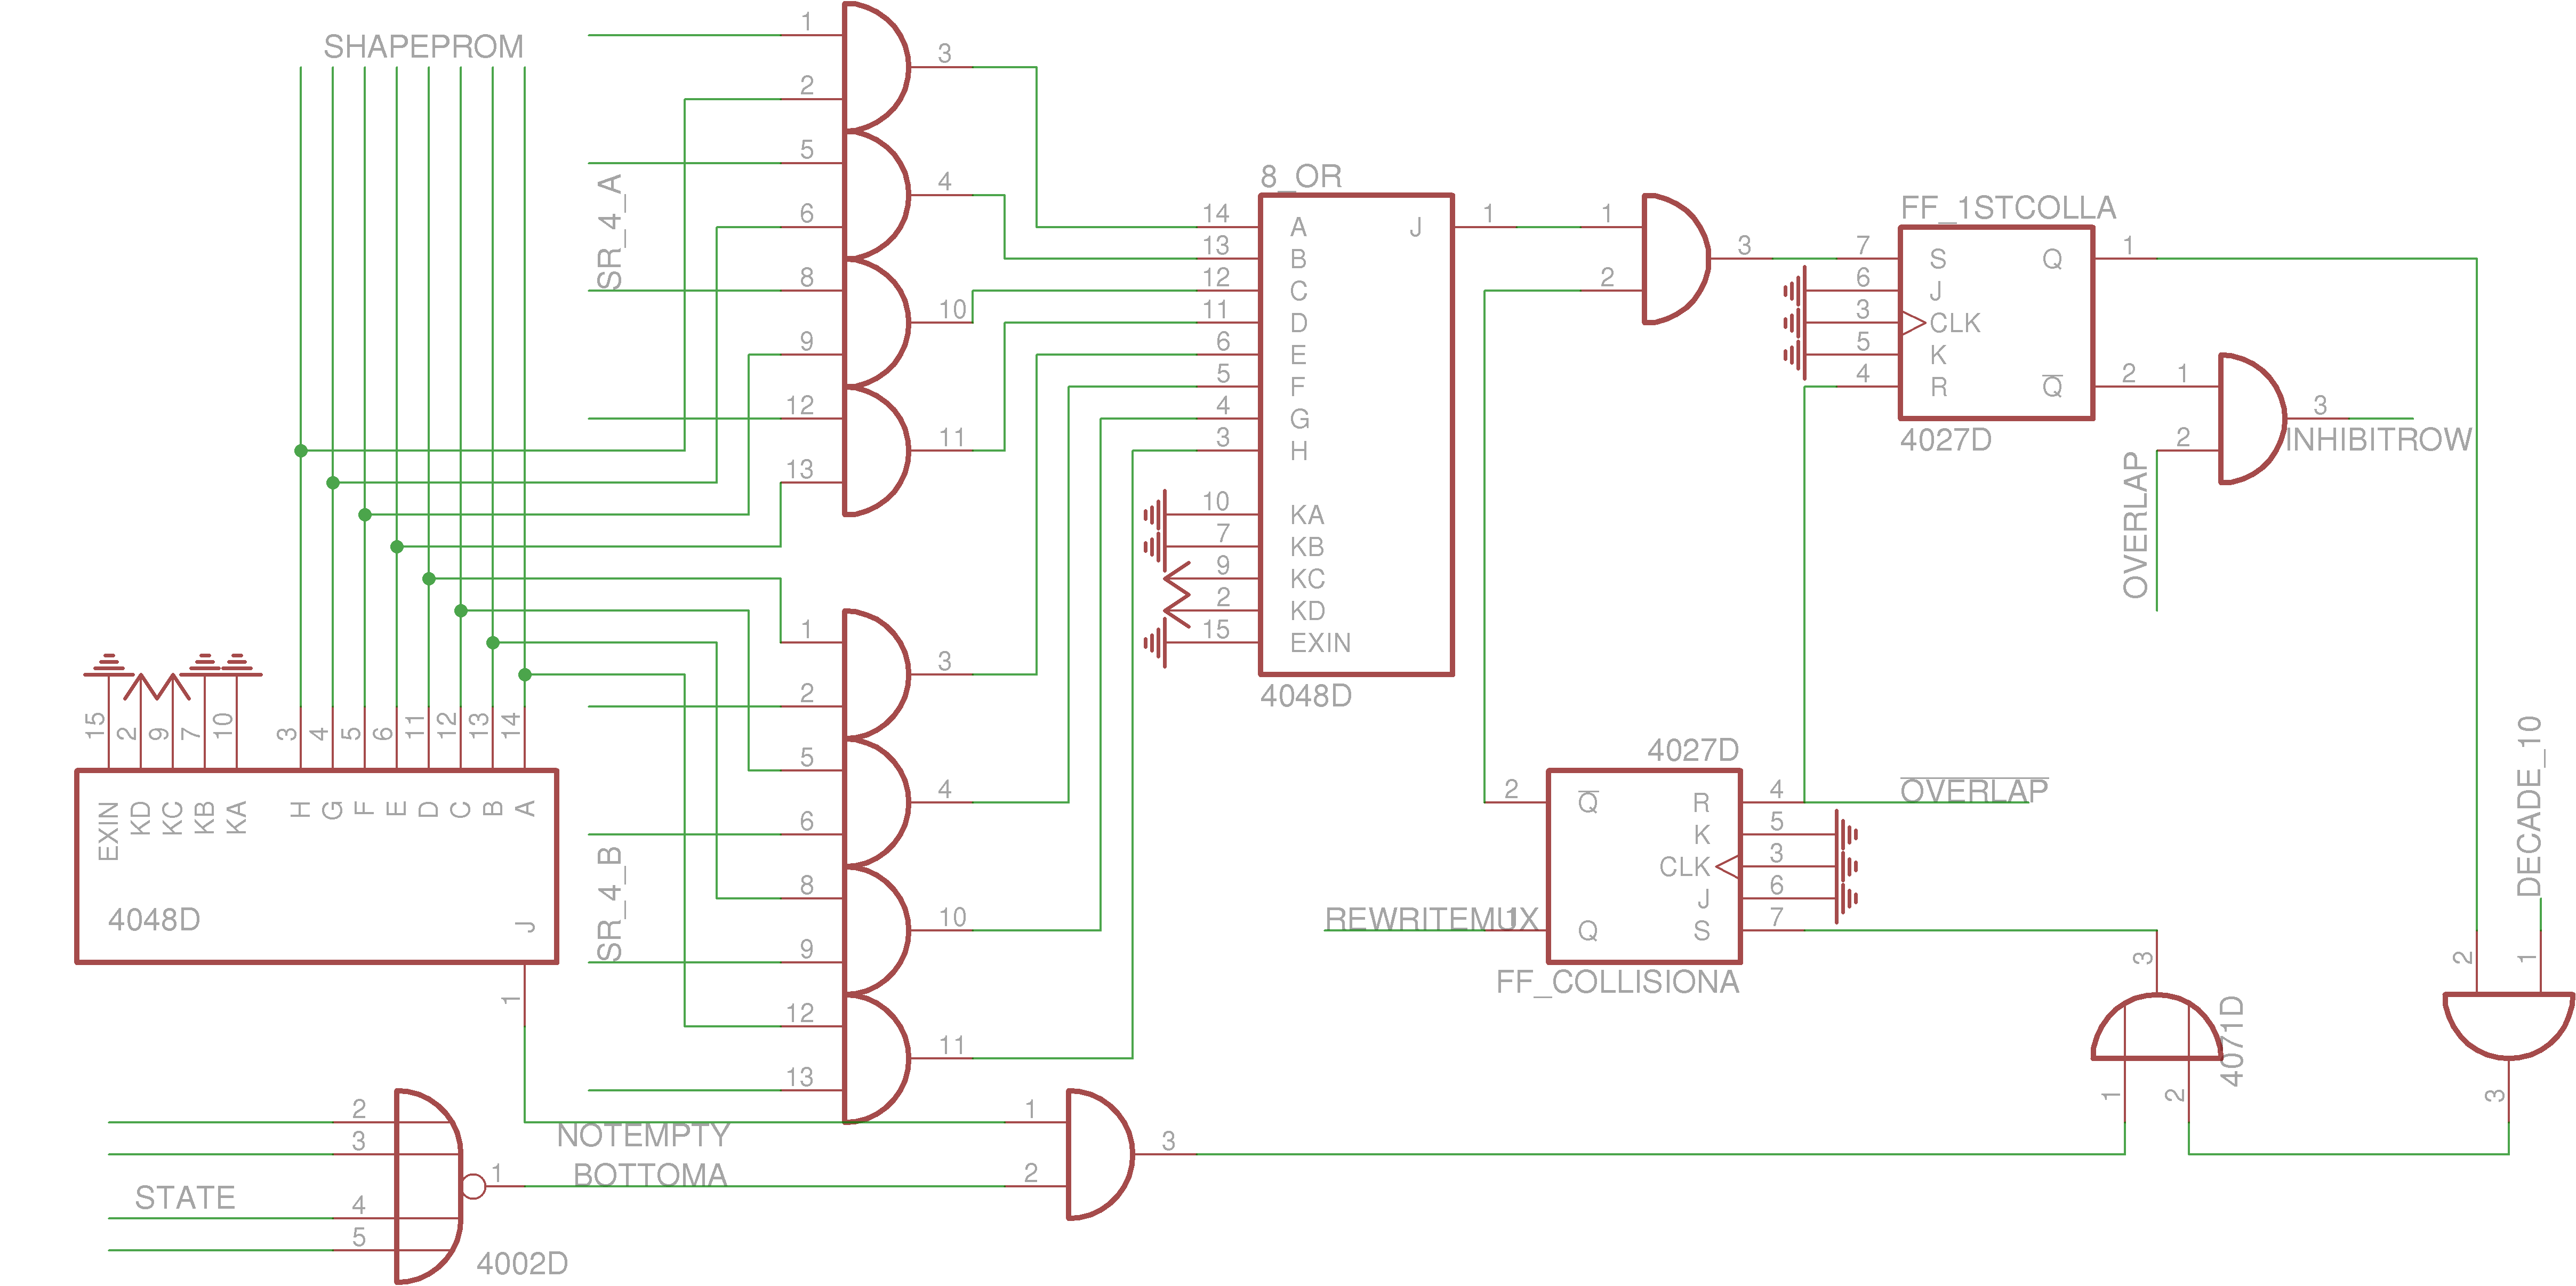
\includegraphics[keepaspectratio=true]{Circuit Diagrams/Collision Logic.png}]{•}
\caption{Collision Logic}
\end{figure}

\end{center}



\end{document}


